\documentclass[11pt,letterpaper]{article}

%%%%%%%%%%%%%%%%%%%%%%%%%%%%
% IMPORTACIÓN DE CONFIGURACIONES
%%%%%%%%%%%%%%%%%%%%%%%%%%%%

\input{configuracion}

%%%%%%%%%%%%%%%%%%%%%%%%%%%%
% INICIO DE DOCUMENTO
%%%%%%%%%%%%%%%%%%%%%%%%%%%%

\begin{document}

%%%%%%%%%%%%%%%%%%%%%%%%%%%%
% ENCABEZADO
%%%%%%%%%%%%%%%%%%%%%%%%%%%%
\begin{center}
    \begin{minipage}{3cm}
    	\begin{center}
    		\includegraphics[height=3.4cm]{Logo_UNAM.png}
    	\end{center}
    \end{minipage}\hfill
    \begin{minipage}{10cm}
    	\begin{center}
    	\textbf{\large Universidad Nacional Autónoma de México}\\[0.1cm]
        \textbf{Facultad de Ciencias}\\[0.1cm]
        \textbf{Nombre de la Materia $|$ Grupo \#\#\#\#}\\[0.1cm]
        Tarea \# - Nombre de la Tarea\\[0.1cm]
        Nombre del estudiante\\[0.1cm]
        \today
    	\end{center}
    \end{minipage}\hfill
    \begin{minipage}{3cm}
    	\begin{center}
    		\includegraphics[height=3.4cm]{Logo_FC.png}
    	\end{center}
    \end{minipage}
\end{center}

\rule{17cm}{0.1mm}

%%%%%%%%%%%%%%%%%%%%%%%%%%%%
% FIN DE ENCABEZADO
%%%%%%%%%%%%%%%%%%%%%%%%%%%%

% ==============================================================================
%% Primer bloque: Indicaciones
% ==============================================================================

\begin{intro}
    \lipsum[2]
\end{intro}

% ==============================================================================
%% Segundo Bloque: Demostraciones
% ==============================================================================

\begin{inciso}{Demostraciones}
- \lipsum[4] 

\begin{teorema}
Aquí va un teorema
\end{teorema}

\begin{demostracion}{P.D. Teorema }
- \lipsum[4] 
\end{demostracion}
\end{inciso}

% ==============================================================================
%% Tercer bloque: Tablas
% ==============================================================================

\begin{inciso}{Tablas}
-    \lipsum[4]


\begin{table}[H]
    \centering
    \begin{tabular}{c*{5}{|c}}
    \multicolumn{3}{c}{}&
    \multicolumn{1}{c}{%
      $\overbrace{\hphantom{(p\land q)\to p}}^{\textbf{(a)}}$%
    }
    &\multicolumn{1}{c}{}&
    \multicolumn{1}{c}{%
      $\overbrace{\hphantom{p\to (p\lor q)}}^{\textbf{(b)}}$%
    }\\[-1ex]
    $p$ & $q$ & $p\land q$ & $(p\land q)\to p$ & $p\lor q$ & $p\to (p\lor q)$\\
    \hline
    T & T & T & T & T & T\\
    T & F & F & T & T & T\\
    F & T & F & T & T & T\\
    F & F & F & T & F & T
    \end{tabular}
    \label{tab:logica}
    \end{table}

\end{inciso}


% ==============================================================================
%% Cuarto bloque: Figuras en Tikz
% ==============================================================================
\begin{inciso}{Figuras en tikz}
-    \lipsum[1]
\\
\begin{center}

    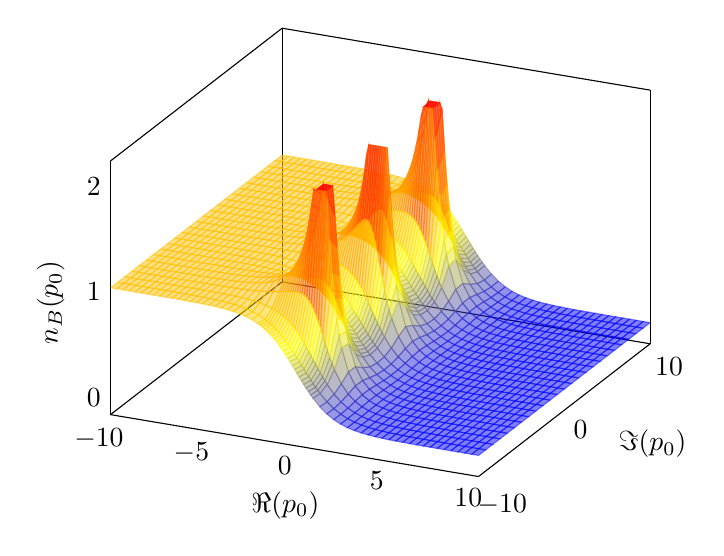
\begin{tikzpicture}
        \begin{axis}[
            xlabel=$\Re(p_0)$,
            ylabel=$\Im(p_0)$,
            zlabel=$n_\text{B}(p_0)$,
            x label style={at={(0.35, 0)}},
            y label style={at={(0.95, 0.15)}},
            shader=flat,
            tickwidth=0pt
            ]
            
            \def\nB{(e^(2*x) - 2*e^x*cos(deg(y)) + 1)^(-1/2)}
            
            \addplot3[surf, opacity=0.5, domain=1:10, y domain=-10:10]{\nB};
            
            \addplot3[surf, opacity=0.5, domain=-10:-2, y domain=-10:10]{\nB};
            
            \addplot3[surf, opacity=0.5, domain=-2:1, y domain=-10:10, restrict z to domain*=0:2]{\nB};
            
        \end{axis}
    \end{tikzpicture}
\end{center}
\end{inciso}

% ==============================================================================
%% Quinto bloque: Observaciones
% ==============================================================================

\begin{inciso}{Observaciones}
- \lipsum[2]
\begin{notas}
\lipsum[4] 
\end{notas}   
\end{inciso}

\newpage

% ==============================================================================
%% Sexto Bloque: Código
% ==============================================================================

\begin{inciso}{Código}
- \lipsum[4]
\end{inciso}

% Comienzo de la figura, que contiene un ejemplo de código en formato de listado
\begin{figure}[H]
    \begin{lstlisting}[
        xleftmargin=0.15in,
        linewidth=0.48\textwidth, 
        basicstyle=\scriptsize\ttfamily
        ] 
__global__
void compute(double comp, int var_1, double var_2,
  double var_3, double var_4, double var_5, 
  double var_6, double var_7, double var_8) {
  if (comp == -1.3857E-36 + var_2) {
    double tmp_1 = +1.3305E12 / var_3;
    comp += -1.7744E-2 * tmp_1;
    comp += cos(var_4 - +1.4014E2 * (var_5 + var_6 * var_7));
    for (int i=0; i < var_1; ++i) {
      comp -= sqrt(var_8 + -1.7976E3);
    }
  }
  printf("%.17g\n", comp);
}
\end{lstlisting}
\end{figure}
% Fin de la figura y del listado del código

% ==============================================================================
%% Séptimo Bloque: Bibliografía
% ==============================================================================

\begin{biblio}
\lipsum[4]
\end{biblio}

\end{document}


    